\documentclass[12pt]{article}
\usepackage[utf8]{inputenc}
\usepackage[T1]{fontenc}
%\usepackage{garamondx}
%\usepackage[garamondx,cmbraces]{newtxmath}
%\usepackage{amsfonts}
\usepackage{amsmath}
\usepackage{txfonts}
\usepackage{amssymb}
\usepackage{pdfpages}
\usepackage[noend]{algpseudocode}
\usepackage{algorithm}
%\usepackage{adjustbox}
%\usepackage{rotating}
\usepackage{tikz}
\usepackage{geometry}
\geometry{
	a4paper,
	total={190mm,265mm}, % a4 is 210 x 297 mm
	left=10mm,
	top=17mm,
}
\usepackage{listings}

\lstdefinestyle{mystyle}{
	backgroundcolor=\color{backcolour},   
	commentstyle=\color{codegreen},
	keywordstyle=\color{magenta},
	numberstyle=\tiny\color{codegray},
	stringstyle=\color{codepurple},
	basicstyle=\ttfamily\footnotesize,
	breakatwhitespace=false,         
	breaklines=true,                 
	captionpos=b,                    
	keepspaces=true,                 
	numbers=left,                    
	numbersep=5pt,                  
	showspaces=false,                
	showstringspaces=false,
	showtabs=false,                  
	tabsize=2
}

\lstset{style=mystyle}

\usepackage{xcolor}
\usepackage{graphicx}
\usepackage{float}

\usepackage[l3]{csvsimple}
\setlength{\parindent}{0pt}
\setlength{\parskip}{1pt}
%New colors defined below
\definecolor{codegreen}{rgb}{0,0.6,0}
\definecolor{codegray}{rgb}{0.5,0.5,0.5}
\definecolor{codepurple}{rgb}{0.58,0,0.82}
\definecolor{backcolour}{rgb}{0.95,0.95,0.92}

\usepackage{subcaption}
\usepackage{hyperref}
\usepackage{enumitem}
\hypersetup{
	colorlinks=true,
	citecolor=codegreen, 
	linkcolor=codegreen,
	filecolor=codepurple,      
	urlcolor=codepurple,}

%\usepackage[autocite=superscript,backend=bibtex,style=nature]{biblatex}
%\bibliography{main}%Import the bibliography file

%%Algorithm
\usepackage{algorithm}
\usepackage{algpseudocode}
\author{SHASHVAT JAIN\\ (2020PHY1114) \and HARSH SAXENA\\ (2020PHY1162)}
\title{\bf {\color{blue}\textbf{Finite Difference Method}\\} } 

\begin{document}	
	\maketitle
	\begin{center}
		\large{\textbf{Assignment No. 11} }
		\vskip 5cm
		{\color{blue}S.G.T.B. Khalsa College, University of Delhi, Delhi-110007, India.\\} 
		\vfill
		Submitted to Dr. Mamta\\
		"32221401 - MATHEMATICAL PHYSICS III"
	\end{center}
	\pagenumbering{gobble}
	
	\newpage
	\tableofcontents
	\newpage
	\pagenumbering{arabic}
	\section{Theory}
	A linear boundary value problem with only one independent variable $ x $, having the Differential equation of the form
	\begin{equation}\label{linear 1D BVP}
		y''(x) + p(x) y'(x) + q(x)y(x) + r(x) = 0 \qquad \forall \quad a\leq x\leq b
 	\end{equation}
 	alongwith Robin boundary conditions, can be solved using the \textbf{Finite Difference Method(FDM)}.
 	
 	The main ordered steps of the finite difference method are:-
 	\begin{enumerate}
 		\item \textit{Domain discretization}:  Discretize the continuous solution domain into a discrete grid, usually taken to be uniform.
 		\item \textit{Differential Equation(DE) $ \rightarrow $ Finite Difference Equation(FDE):} Replacing the derivatives in the differential equation with their appropriate Difference Quotients or finite difference approximations to obtain the Finite difference equation(FDE) over the discretized domain.
 		\item \textit{Linear Boundary Value Problem(BVP) $ \rightarrow $ System of Linear Equations($ A\vec{y} = b $)}: Apply the FDE to each \textit{node} in the discretized grid to obtain a system of linear equations with unknowns being the value of the dependent variable $ y $ at these nodes.
 		\item \textit{Solving the system for $ y $}: Solve the system of linear equations for the value of the dependent $ y $ at nodes in the discretized domain.
 	\end{enumerate}
 	Given a very fine grid(with many nodes) and some clue about the nature of the solution of the BVP in the continuous domain, you can interpolate the approximate expression for $ y $ from the values of $ y $ obtained at nodes by using appropriate interpolation methods.
 	
 	\subsection[Discretization]{\textit{Domain Discretization}}
 	To apply our finite difference equation, we need to first discretize our domain.
 	To discretize our continuous domain $ [a,b] $, break the domian into $ n $ several regions or subintervals of equal length $ h := (b-a)/n $ to obtain a structure that resembles a \textit{uniform grid}, we will only work on the points that seperate these subintervals\\ $ x_i := a + ih \quad i=0,1,2\dots,n-1,n $ instead of the entire continuous domain.
 	\begin{figure}[h]
 		\centering
 		
 		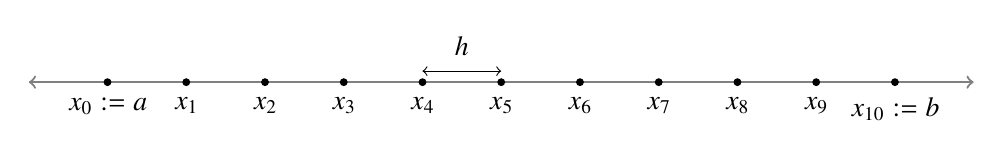
\begin{tikzpicture}
 			\coordinate (H) at (4.5,6pt);
 			\draw[thick,color=gray,<->] (-1,0) -- (11,0);
 			\draw[fill=black] (0 cm,0) circle (1.2pt) (0 cm,-2pt) node[anchor=north] {$x_{0}:= a$};
 			\draw[fill=black] (10 cm,0) circle (1.2pt) (10 cm,-2pt) node[anchor=north] {$x_{10}:= b$};
 			\foreach \x  in {1,2,3,4,5,6,7,8,9}
 			\draw[fill=black] (\x cm,0) circle (1.2pt) (\x cm,-2pt) node[anchor=north] {$x_{\x}$};
 			\draw[thin,<->] (4,4pt) -- (5,4pt);%
 			\node[anchor=south] at (H) {$h$};
 		\end{tikzpicture}
 		\caption{\small 1D grid with 11 nodes and a meshsize h}
 	\end{figure}
 
 	\subsection{\textit{Differential Equation(DE) $ \rightarrow $ Finite Difference Equation(FDE)}}
 	\subsubsection{Finite Difference Approximations}
 	The quality of the solution depends on the quality of approximations made to the derivatives. The act of making such approximations to the derivatives itself induces errors in our solution at the nodes, such error is called \textbf{truncation error} which will be talked upon more in the coming sections.
 	
 	
 	The first order derivative can be defined as,
 	{\raggedright 
 		\begin{align*}
 			&\text{} \hspace{1cm} y'_i := y'(x_i) := \lim_{h \to 0} \frac{y_{i+1} - y_i}{h}  \\
 			&\text{or,} \hspace{1cm} y'_i := \lim_{h \to 0} \frac{y_{i} - y_{i-1}}{h}  \\
 			&\text{or,} \hspace{1cm} y'_i := \lim_{h \to 0} \frac{y_{i+1} - y_{i-1}}{2h}  
 		\end{align*}
 	}
 	
 	Finite difference approximations are obtained by dropping the limit and can be written as, 
 	
 	\begin{flalign*}
 		&\text{Forward Difference} \hspace{1cm} y'_i \approx \frac{y_{i+1} - y_i}{h} \equiv \delta^+_{x} y_i  \\
 		&\text{Backward Difference} \hspace{1cm} y'_i \approx \frac{y_{i} - y_{i-1}}{h} \equiv \delta^-_{x} y_i \\
 		&\text{Central Difference} \hspace{1cm} y'_i \approx \frac{y_{i+1} - y_{i-1}}{2h} \equiv \delta_{2x} y_i 
 	\end{flalign*}
 	
 	Where $\delta^+_{x} , \delta^-_{x} , \delta_{2x}$ are called the \textbf{finite diference operators} for approximating \textbf{first-order derivatives} and their expansion is called the \textbf{finite difference quotient}, each representing forward,backward and centered respectively.\\ \textbf{Note that the order of finite difference operators is the order of $ h $ in the trunction error they accompany and NOT the order of the derivative they apporximate.} \\\\
 	Finite difference Quotients to higher order derivatives can also be obtained using these these operators,
 	\begin{align*}
 		y''_i &= \lim_{h \to 0} \frac{y'(x_i+\frac{h}{2}) - y'(x_i-\frac{h}{2})}{h} \\
 		&= \lim_{h \to 0} \frac{1}{h} \left[{\frac{y(x_i+h) - y(x_i)}{h} - \frac{(y(x)- y(x_i-h))}{h}}\right]\\
 		&= \lim_{h \to 0}\frac{y_{i+1}-2 y_i + y_{i-1}}{h^2} \\
 		&\approx \boxed{\delta^2_x y_i \equiv \frac{1}{h^2}(y_{i+1}-2 y_i + y_{i-1})} \hspace{1cm} \text{[Central difference for second-order derivative]}
 	\end{align*}
 	
 	
 	\subsubsection{Local Truncation Error of Finite Difference Approximations}
 	The \textit{"error"} that accompanies \textit{"approximations"} in the method must also be acccounted for. In this section, the truncation error in the derivative approximations is ascertained which will later help us deduce the error in PDE's solved using these approximations.
 	\\[2mm]
 	\textbf{The local truncation error for derivative approximations} is defined here as the difference between the exact value of the derivate and the approximated value at node $i$, it can be calculated using Taylor series expansions about $i$,\\[2mm]
 	For Forward difference operator,%\autocite{mitocw}%\cite{thomas2013numerical}
 	\begin{align*}
 		\tau &\equiv \delta _ x^{+} y_i - {y'}|_ i \\
 		&= \frac{1}{h}\left( y_ {i+1} - y_{i}\right) - {y'}|_i \\
 		&= \frac{1}{h}\left[ \left( y_i + h{y'}|_ i + \frac{1}{2}(h)^2{y''}|_ i + O((h)^3)\right) - y_i \right] - {y'}|_ i \\
 		&= \frac{1}{2}h{y''}|_ i + O((h)^2) = O(\Delta x)
 	\end{align*}
 	For Backward difference operator, 
 	\begin{align*}
 		\tau &\equiv \delta _ x^{-} y_i - {y'}|_ i \\
 		&= \frac{1}{h}\left( y_i - y_{i-1}\right) - {y'}|_i \\
 		&= \frac{1}{h}\left[ y_i - \left( y_i - h{y'}|_ i + \frac{1}{2}(h)^2{y''}|_ i + O((h)^3)\right)\right] - {y'}|_ i \\
 		&= -\frac{1}{2}h{y''}|_ i + O((h)^2) = O(\Delta x)  
 	\end{align*}
 	For Central difference operator,
 	\begin{align*}
 		\tau &\equiv \delta _ {2x} y_i - {y'}|_ i \\
 		&= \frac{1}{2h}\left( y_{i+1} - y_{i-1}\right) - y'_i \\
 		&= \frac{1}{2h}\Bigg[ \left( y_i + h{y'}|_ i + \frac{1}{2}(h)^2{y''}|_ i + \frac{1}{6}(h)^3{y_{xxx}}|_ i + \frac{1}{12}(h)^4{y_{xxxx}}|_ i + O((h)^5)\right) \\
 		%&\qquad - \left( y_i - h{y'}|_ i + \frac{1}{2}(h)^2{y''}|_ i - \frac{1}{6}(h)^3{y_{xxx}}|_ i + \frac{1}{12}(h)^4{y_{xxxx}}|_ i +O((h)^5)\right)\Bigg] - {y'}|_ i \\
 		%&= -\frac{1}{6}h^2 y_{xxx_ i} + O((h)^4) = O(h^2)
 	\end{align*}
 	where in the above expressions we assume that the Higher order derivatives of $y$ at $i$ are well defined. For a fairly small $h$ (less than 1) we can confidently say that $O(h^2)$ is samller than $O(h)$%
 	\footnote{The definition of the "big $O$" notation says that if for given functions $f(x)$ and $g(x)$ for $x \in S$ where S is some subset of $\mathbf{R}$, there exists a positive constant A such that $|f(x)| \leq A|g(x)|$ $\forall \, x \in S$, we say that $f(x)$ is the "big $O$" of $g(x)$ or that $f(x)$ is of order of $g(x)$, mathematically given by $f(x) = O(g(x))$}. Thus we note that the centered difference approximation (second-order accurate) approximates the derivative more accurately than either of the \textit{one-sided diferences} which are first-order accurate.\footnote{Forward and Backward differences are also called one-sided differences} 	
 	Similarly, Approximation of second-order derivative,
 	\begin{align*}
 		\tau &\equiv \delta^2_x y_i - y''|_i \\
 		&= \frac{1}{h^2}(y_{i+1}-2 y_i + y_{i-1})  - y''|_i \\
 		&= \frac{1}{h^2}\Bigg[ \left( y_i + h{y'}|_ i + \frac{1}{2}h^2{y''}|_ i + \frac{1}{6}h^3{y'''}|_ i + \frac{1}{12}h^4{y''''}|_ i + O(h^5)\right) - 2 y_i +\\ &\qquad\qquad \left( y_i - h{y'}|_ i + \frac{1}{2}h^2{y''}|_ i - \frac{1}{6}h^3{y'''}|_ i + \frac{1}{12}h^4{y''''}|_ i +O(h^5)\right)\Bigg] - {y''}|_ i \\
 		&= O(h^2)
 	\end{align*}
 	\subsection{\textit{Obtaining FDE}}
 	
 	Since the central difference approximations yield the least error, we substitute teh central difference approximations in differential equation \ref{linear 1D BVP} for any interior point $ x_i ; i = 1,2,3,\dots n-1$ in the grid to obtain,
 	\begin{align}\label{Difference Equation}
 		 \frac{1}{h^2}(y_{i+1}-2 y_i + y_{i-1}) + p_i \frac{y_{i+1} - y_{i-1}}{2h} + q_i y_i + r_i &= 0 \nonumber\\
 		 \implies y_{i+1}\left(1+\frac{h p_i}{2}\right) + y_{i}\left(-2+q_i h^2\right)+y_{i-1}\left(1-\frac{h p_i}{2}\right) &= -h^2r_i 
 	\end{align}
 	The truncation error that accompanies the above obtained FDE is the truncation error in the derivates, that is, $ O(h^2) $.
 	\subsection{Robin Boundary Conditions}
	
	Since we are dealing with a closed interval $ [a,b] $, the differential equation \ref{linear 1D BVP} must also hold at the end points, in addition to it, we are constrained further with two more equations, one for each boundary point,
	\begin{align}\label{robin}
		\alpha_1 y_0 + \alpha_2 y'_0 &= \alpha_3 \\
		\beta_1 y_n + \beta_2 y'_n &= \beta_3
	\end{align}
	To obtain a corresponding difference form for the above boundary equations we assume the existence of ficticious variables $ y_{-1} $ and $ y_{n+1} $, 
	\begin{align}\label{robin_DE}
		\alpha_1 y_0 + \alpha_2 \frac{y_{1} - y_{-1}}{2h} &= \alpha_3 \implies \boxed{y_{-1} = y_1 + \frac{2h}{\alpha_2}\left(\alpha_1 y_0 - \alpha_3\right)} \\
		\beta_1 y_n + \beta_2 \frac{y_{n+1} - y_{n-1}}{2h} &= \beta_3 \implies \boxed{y_{n+1} = y_{n-1} - \frac{2h}{\beta_2}\left(\beta_1 y_n - \beta_3\right)}
	\end{align}
	
	\subsection{\textit{Linear Boundary Value Problem(BVP) $ \rightarrow $ System of Linear Equations($ A\vec{y} = b $)}}
	Since \ref{Difference Equation} holds for all $ i = 1,2,3,\dots n-1 $, we obtain the system,
	\begin{equation} \label{sys1}
	 \left[ \begin{matrix}
		l_1 & d_1 & u_1 & 0 &\cdots &\cdots&\cdots& 0\\
		0&l_2 & d_2 & u_2 &0 &\cdots&\cdots& 0\\
		0&0 & \ddots & \ddots &\ddots &\cdots&\cdots & \vdots\\
		\vdots&\cdots&0&l_k & d_k & u_k &\cdots& \vdots\\
		\vdots&\cdots&\cdots&\ddots & \ddots & \ddots &\ddots& \vdots\\
		0&\cdots&\cdots& \cdots&0 & l_{n-1} &d_{n-1}& u_{n-1}\\
		\end{matrix} \right]
	\left[ \begin{matrix}
		y_0\\
		y_1\\
		y_2\\
		\vdots\\
		\vdots\\
		y_{n-1}\\
		y_{n}\\
	\end{matrix} \right] =
		\left[ \begin{matrix}
		- h^2 r_1\\
		- h^2 r_2\\
		- h^2 r_3\\
		\vdots\\
		- h^2 r_{n-2}\\
		- h^2 r_{n-1}\\
	\end{matrix} \right]
	\end{equation}
	where,
	\begin{equation*}
		d_k = -2+q_k h^2 \qquad\qquad u_k = 1+\frac{h p_k}{2} \qquad\qquad l_k = 1-\frac{h p_k}{2} \qquad k = 0,1,2,\cdots n-1,n
	\end{equation*}
	
	clearly one observes, the system \ref{sys1} has $ n-1 $ equations and $ n+1 $ unknowns, We have to also account for the equations obtained at the boundaries, that is, $ i = 0,n $
	
	For $ i = 0 $
	we have the relation from the FDE,
	\begin{equation}\label{fde_a}
		 y_{1}\left(1+\frac{h p_0}{2}\right) + y_0\left(-2+q_0 h^2\right)+y_{-1}\left(1-\frac{h p_0}{2}\right) = -h^2r_0 
	\end{equation}
	but we also have to constraint \ref{robin_DE} (\textbf{NOTE: we assume $ \alpha_2 \neq 0 $, we will learn how to deal with this condition soon.}), combining the two we get,
	\begin{equation}\label{i=0}
		2 y_1 + y_0 \left(d_0 + \frac{2h \alpha_1 l_0}{\alpha_2}\right) = -h^2r_0 + \frac{2h \alpha_3 l_0}{\alpha_2}
	\end{equation}
	Similarly, For $ i = n $ we obtain,
	\begin{equation}\label{i=n}
		2 y_{n-1} + y_n \left(d_n - \frac{2h \beta_1 u_n}{\beta_2}\right) = -h^2r_n - \frac{2h \beta_3 u_n}{\beta_2}
	\end{equation}
	Adding equations \ref{i=0} and \ref{i=n} to the system \ref{sys1}, we obtain the system,
		\begin{equation} \label{sys2}
		\left[ \begin{matrix}
			d_0 + \frac{2h \alpha_1 l_0}{\alpha_2} & 2 & 0 & \cdots &\cdots &\cdots&\cdots& 0\\
			l_1 & d_1 & u_1 & 0 &\cdots &\cdots&\cdots& \vdots\\
			0&l_2 & d_2 & u_2 &0 &\cdots&\cdots& \\
			&0 & \ddots & \ddots &\ddots &\ddots&\cdots & \vdots\\
			\vdots&\cdots&0&l_k & d_k & u_k &\ddots& \vdots\\
			\vdots&\cdots&\cdots&\ddots & \ddots & \ddots &\ddots& 0\\
			&\cdots&\cdots& \cdots&\ddots & l_{n-1} &d_{n-1}& u_{n-1}\\
			0&\cdots&\cdots& \cdots&\cdots & 0 & 2 & d_n - \frac{2h \beta_1 u_n}{\beta_2} \\
		\end{matrix} \right]
		\left[ \begin{matrix}
			y_0\\
			y_1\\
			y_2\\
			\vdots\\
			\vdots\\
			\vdots\\
			y_{n-1}\\
			y_{n}\\
		\end{matrix} \right] =
		\left[ \begin{matrix}
			-h^2r_0 + \frac{2h \alpha_3 l_0}{\alpha_2} \\
			- h^2 r_1\\
			- h^2 r_2\\
			- h^2 r_3\\
			\vdots\\
			- h^2 r_{n-2}\\
			- h^2 r_{n-1}\\
			-h^2r_n - \frac{2h \beta_3 u_n}{\beta_2}\\
		\end{matrix} \right]
	\end{equation}
	This system has $ n+1 $ equations and $ n+1 $ unknowns, but the system fails at $ \alpha_2= 0 $ or $\beta_2 = 0 $.
	when $ \alpha_2 = 0 $ or $\beta_2 = 0 $ we see that the Robin boundary conditions \ref{robin} reduce to Dirichlet boundary conditions,
	\begin{align}\label{dirichlet1}
		 y_0 &= \alpha_3/\alpha_1 \\
		 y_n &= \beta_3/\beta_1 \label{dirichlet2}
	\end{align}
	Therefore we obtain a system combining \ref{dirichlet1},\ref{dirichlet2} and \ref{sys1},
	\begin{equation} \label{sys3}
	\left[ \begin{matrix}
		1 & 0 & 0 & \cdots &\cdots &\cdots&\cdots& 0\\
		l_1 & d_1 & u_1 & 0 &\cdots &\cdots&\cdots& 0\\
		0&l_2 & d_2 & u_2 &0 &\dots&\cdots& 0\\
		0&0 & \ddots & \ddots &\ddots &\ddots&\cdots & \vdots\\
		\vdots&\cdots&0&l_k & d_k & u_k &\ddots& \vdots\\
		\vdots&\cdots&\cdots&\ddots & \ddots & \ddots &\ddots& \vdots\\
		0&\cdots&\cdots& \cdots&\ddots & l_{n-1} &d_{n-1}& u_{n-1}\\
		0&\cdots&\cdots& \cdots&\cdots & \cdots & 0 & 1 \\
	\end{matrix} \right]
	\left[ \begin{matrix}
		y_0\\
		y_1\\
		y_2\\
		\vdots\\
		\vdots\\
		\vdots\\
		y_{n-1}\\
		y_{n}\\
	\end{matrix} \right] =
	\left[ \begin{matrix}
		\alpha_3/\alpha_1 \\
		- h^2 r_1\\
		- h^2 r_2\\
		- h^2 r_3\\
		\vdots\\
		- h^2 r_{n-2}\\
		- h^2 r_{n-1}\\
		\beta_3/\beta_1\\
	\end{matrix} \right]
	\end{equation}
	Therefore in general we obtain, 
	\begin{equation} \label{sys_gen}
		\left[ \begin{matrix}
			a_{11} & a_{12} & 0 & \cdots &\cdots &\cdots&\cdots& 0\\
			l_1 & d_1 & u_1 & 0 &\cdots &\cdots&\cdots& 0\\
			0&l_2 & d_2 & u_2 &0 &\cdots&\cdots& 0\\
			0&0 & \ddots & \ddots &\ddots &\ddots&\cdots & \vdots\\
			\vdots&\cdots&0&l_k & d_k & u_k &\ddots& \vdots\\
			\vdots&\cdots&\cdots&\ddots & \ddots & \ddots &\ddots& \vdots\\
			0&\cdots&\cdots& \cdots&\ddots & l_{n-1} &d_{n-1}& u_{n-1}\\
			0&\cdots&\cdots& \cdots&\cdots & \cdots & a_{n,n-1} & a_{n,n} \\
		\end{matrix} \right]
		\left[ \begin{matrix}
			y_0\\
			y_1\\
			y_2\\
			\vdots\\
			\vdots\\
			\vdots\\
			y_{n-1}\\
			y_{n}\\
		\end{matrix} \right] =
		\left[ \begin{matrix}
			b_0 \\
			- h^2 r_1\\
			- h^2 r_2\\
			- h^2 r_3\\
			\vdots\\
			- h^2 r_{n-2}\\
			- h^2 r_{n-1}\\
			b_n \\
		\end{matrix} \right]
	\end{equation}
	where,
	\begin{equation}\label{edges}
		a_{11} = \left\{ \begin{array}{cr}
				1 &; \alpha_2 = 0 \\[3mm]
			\displaystyle	d_0 + \frac{2h \alpha_1 l_0}{\alpha_2} &; \alpha_2 \neq 0 \\
			\end{array} \right.
		\qquad\qquad
		a_{12} = \left\{ \begin{array}{cr}
			0 &; \alpha_2 = 0 \\[3mm]
			2 &; \alpha_2 \neq 0 \\
		\end{array} \right.
		\qquad\qquad
		b_0 = \left\{ \begin{array}{cr}
			\alpha_3/\alpha_1 &; \alpha_2 = 0 \\[3mm]
			\displaystyle -h^2r_0 + \frac{2h \alpha_3 l_0}{\alpha_2} &; \alpha_2 \neq 0 \\
	\end{array} \right.
	\end{equation}
		\begin{equation}\label{edges2}
		a_{nn} = \left\{ \begin{array}{cr}
			1 &; \beta_2 = 0 \\[3mm]
			\displaystyle d_n - \frac{2h \beta_1 u_n}{\beta_2} &; \beta_2 \neq 0 \\
		\end{array} \right.
		\qquad\qquad
		a_{n+1,n} = \left\{ \begin{array}{cr}
			0 &; \beta_2 = 0 \\[3mm]
			2 &; \beta_2 \neq 0 \\
		\end{array} \right.
		\qquad\qquad
		b_n = \left\{ \begin{array}{cr}
			\beta_3/\beta_1 &; \beta_2 = 0 \\[3mm]
			\displaystyle -h^2r_n - \frac{2h \beta_3 u_n}{\beta_2} &; \beta_2 \neq 0 \\
		\end{array} \right.
	\end{equation}
	System \ref{sys_gen} can be solved to obtain $ \vec{y} $
	\newpage
	\section{Algorithm}
	\begin{algorithm}[H]
		\centering
		\caption{Crout factorization for tridiagonal linear systems}
		\begin{algorithmic}
			\Procedure{Crout}{n,A,b} \hline \\
			\State Input: n is the shape of the marix A,A contains the tridiagonal system,b is a vector which is used to evaluate x in Ax = b.
			\State Output: Returns,x
			\hline
			\Comment{Set up Lz = b and solve for z}
			\State $l_{11} = a_{11}$
			\State $u_{12} = a_{12}/l_{11}$ 
			\State $z_{1} = b_{1}/l_{11}$
			
			\For{ $i = 2,3\dots N-1$ }
			\State ${\displaystyle l_{i,i-1} = a_{i,i-1}}$
			\Comment{$i_{th}$ row of L}
			\State ${\displaystyle l_{i,i} = a_{i,i} - l_{i,i-1}u_{i-1,i}}$
			\State ${\displaystyle u_{i,i+1} = a_{i,i+1}/l_{i,i}}$
			\Comment{$(i+1)_{th}$ column of U}
			\State ${\displaystyle z_{i} = (b_{i} - l_{i,i-1}z_{i-1})/l_{i,i} }$
			\EndFor
			\State Set
			\State ${\displaystyle l_{n,n-1} = a_{n,n-1}}$
			\Comment{$n_{th}$ row of L}
			\State ${\displaystyle l_{n,n} = a_{n,n} - l_{n,n-1}u_{n-1,n}}$
			\State ${\displaystyle z_{n} = (b_{n} - l_{n,n-1}z_{n-1})/l_{n,n} }$
			\State Set $x_{n} = z_{n}$
			\For{ $i = N-1,N \dots,1$ }
			\State ${\displaystyle x_{i} = z_{i} - u_{i,i+1}x_{i+1}}$
			\EndFor
			\State \textbf{Return} $x_{1},x_{2},\dots$
			\State EXIT
			\EndProcedure
		\end{algorithmic} 
	\end{algorithm}
	\section{Results and Analysis}
	For the boundary value problem,
	\begin{equation}\label{bvp1}
		-y'' + \pi^2 y =2\pi^2\sin(\pi x) \qquad; \qquad 0 \leq x \leq 1
	\end{equation}
	\begin{equation*}\label{bvp1bc}
		y(0) = y(1) = 0
	\end{equation*}
	and exact solution given to be,
	\begin{equation}\label{bvp1exac}
		y^{\text{exact}} = \sin(\pi x)
	\end{equation}
	
	\begin{table}[h]
		\centering
		\caption{Data obtained for boundary value problem \ref{bvp1} with $ N = 3 $}
		\csvautotabular{datE_fdm_N3.csv}
	\end{table}
	\begin{table}[h]
		\centering
		\caption{Data obtained for boundary value problem \ref{bvp1} with $ N = 8 $}
		\csvautotabular{dat1.csv}
	\end{table}

	For the second boundary value problem,
	\begin{equation}\label{bvp2}
		y'' + y = \sin(3 x) \qquad; \qquad 0 \leq x \leq \frac{\pi}{2}
	\end{equation}
	\begin{align*}\label{bvp2bc}
		y(0) + y'(0) &= -1\\
		y'(\pi/2) = 1
	\end{align*}
	and exact solution given to be,
	\begin{equation}\label{bvp2exac}
		y^{\text{exact}} = \frac{3}{8}\sin(x) - \cos(x) - \frac{1}{8}\sin(3x)
	\end{equation}
	\begin{table}[H]
		\centering
		\caption{Data obtained for boundary value problem \ref{bvp2} with $ N = 3 $}
		\csvautotabular{datE_fdm_bvp2_N3.csv}
	\end{table}
	\begin{table}[H]
		\centering
		\caption{Data obtained for boundary value problem \ref{bvp2} with $ N = 8 $}
		\csvautotabular{datE_fdm_bvp2_N8.csv}
	\end{table}
	\subsection{Numerical solution scatter plots alongwith exact solution}
	\begin{figure}[H]
		\centering
		\caption{Numerical and Exact solutions for BVP \ref{bvp1}}
		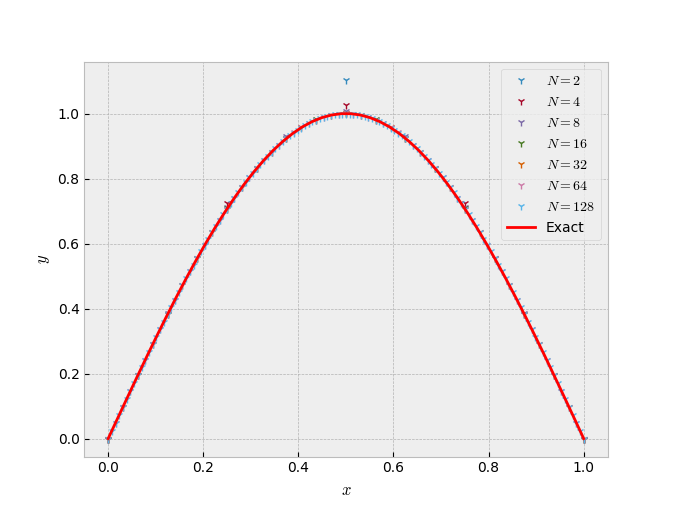
\includegraphics{/home/planck/sdev/mp-3/reports/BVP/bvp1_soln.png}
	\end{figure}

	\begin{figure}[H]
		\centering
		\caption{NUmerical and Exact solutions for BVP \ref{bvp2}}
		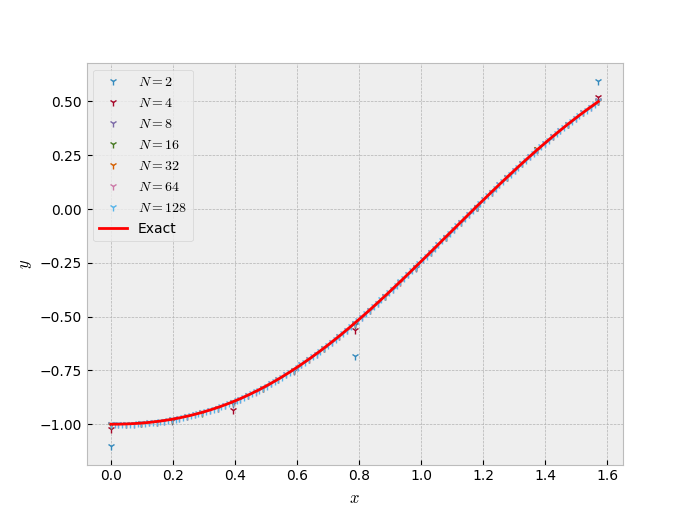
\includegraphics{/home/planck/sdev/mp-3/reports/BVP/bvp2_soln.png}
	\end{figure}
	\newpage
	\subsection{Validating the $ ln(E) $ vs $ ln(N) $ behaviour}
	We know that the truncation error that that accompanies the FDE gives a lower bound on the error in our $ y_{num} $ values,
	\begin{align}\label{key}
		ln(E_{max}) &= ln(O(h^2)) \qquad \nonumber\\ &\text{Given that the error due to rounding off is neglibible in comparison to truncation,$O(h^2) := h^2$}\nonumber\\
		&= ln((b-a)^2N^{-2}) \nonumber\\
		&= -2 ln((b-a)^{-1}N) \nonumber \\
		&= -2 ln(N) - ln(b-a)
	\end{align}
	\begin{figure}[H]
		\centering
		\caption{$ln(E)$ vs $ln(N)$ graph for $N = 2^k \quad k =1,2,\dots,6$ for BVP \ref{bvp1}}
		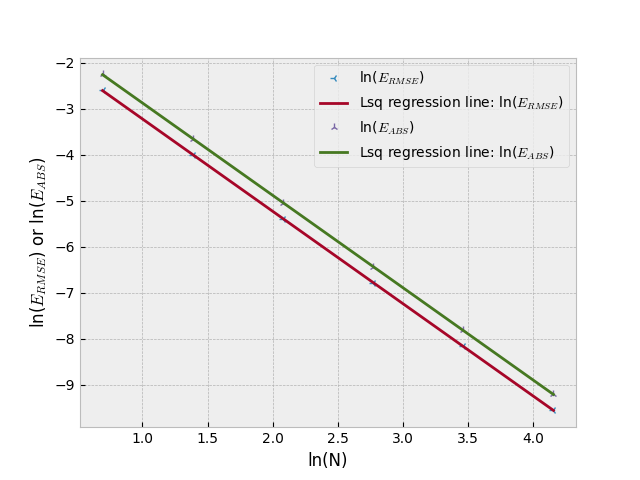
\includegraphics{/home/planck/sdev/mp-3/reports/BVP/bvp1_lnE.png}
	\end{figure}
	
	\begin{figure}[H]
		\centering
		\caption{$ln(E)$ vs $ln(N)$ graph for $N = 2^k \quad k =1,2,\dots,6$ for BVP \ref{bvp2}}
		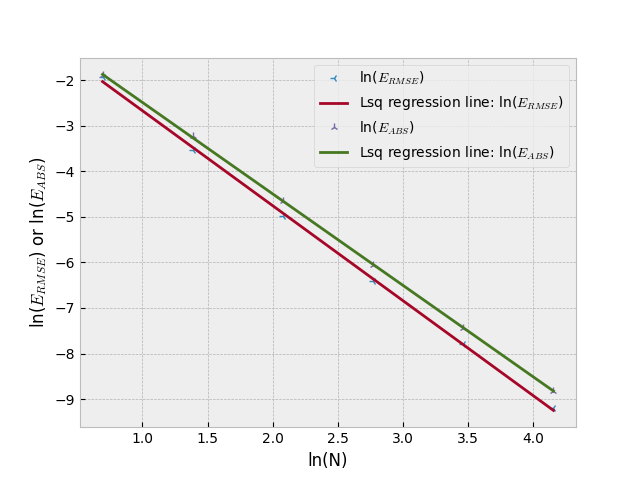
\includegraphics{/home/planck/sdev/mp-3/reports/BVP/bvp2_lnE.png}
	\end{figure}
	
	Slope of the regression trend lines for max absolute error $E_{ABS}$ obtained by Least-squares regression is $\approxeq -2.0042476$ and $ -2.00700754$ for BVP \ref{bvp1} and \ref{bvp2} respectively, this validates our truncation error to be of order 2.
	
\end{document}